\documentclass[tikz,border=6pt]{standalone}
\usepackage{amsmath}
\usetikzlibrary{arrows.meta,positioning}
\begin{document}
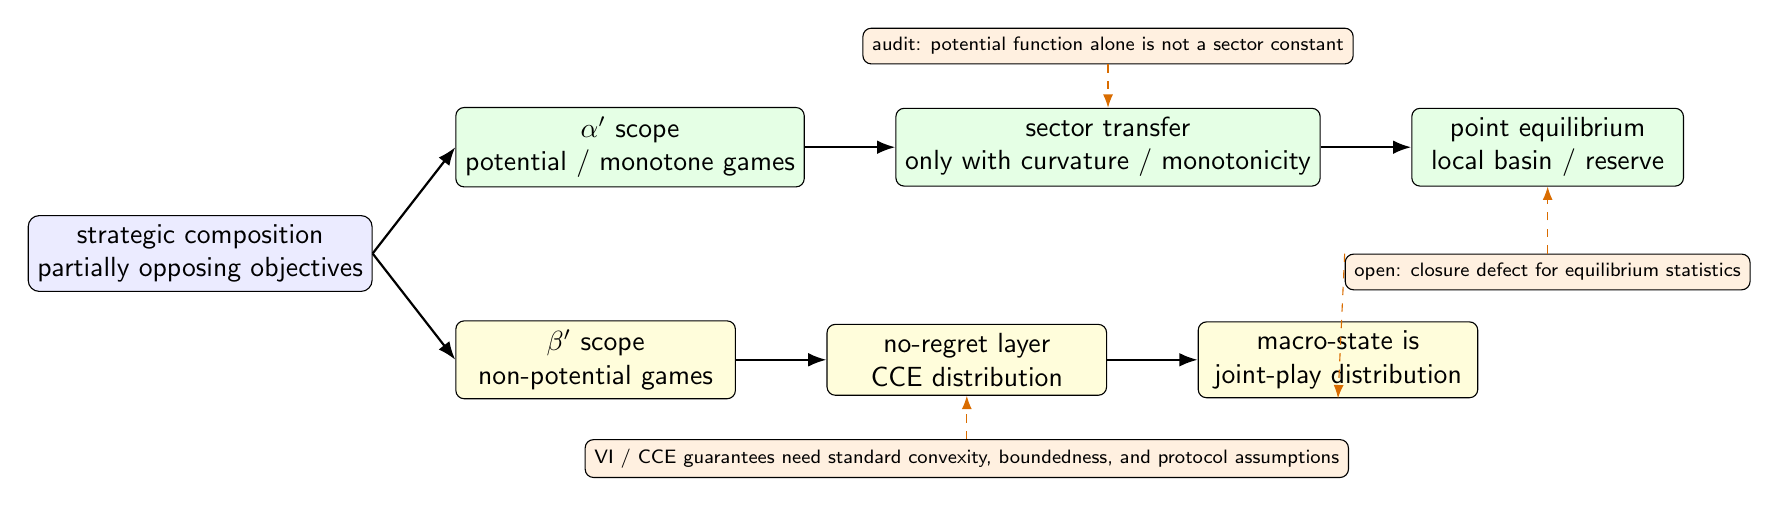
\begin{tikzpicture}[
  font=\sffamily,
  >=Latex,
  root/.style={draw, rounded corners=4pt, fill=blue!8, align=center, minimum width=3.5cm, minimum height=0.95cm},
  path/.style={draw, rounded corners=3pt, fill=green!10, align=center, minimum width=3.45cm, minimum height=0.85cm},
  weak/.style={draw, rounded corners=3pt, fill=yellow!14, align=center, minimum width=3.55cm, minimum height=0.85cm},
  warn/.style={draw, rounded corners=3pt, fill=orange!12, align=center, font=\sffamily\scriptsize}
]

\node[root] (strategic) {strategic composition\\partially opposing objectives};

\node[path, right=1.05cm of strategic, yshift=1.35cm] (alpha) {$\alpha'$ scope\\potential / monotone games};
\node[path, right=1.15cm of alpha] (sector) {sector transfer\\only with curvature / monotonicity};
\node[path, right=1.15cm of sector] (point) {point equilibrium\\local basin / reserve};

\node[weak, right=1.05cm of strategic, yshift=-1.35cm] (beta) {$\beta'$ scope\\non-potential games};
\node[weak, right=1.15cm of beta] (cce) {no-regret layer\\CCE distribution};
\node[weak, right=1.15cm of cce] (dist) {macro-state is\\joint-play distribution};

\draw[->, thick] (strategic.east) -- (alpha.west);
\draw[->, thick] (alpha.east) -- (sector.west);
\draw[->, thick] (sector.east) -- (point.west);

\draw[->, thick] (strategic.east) -- (beta.west);
\draw[->, thick] (beta.east) -- (cce.west);
\draw[->, thick] (cce.east) -- (dist.west);

\node[warn, above=0.55cm of sector, minimum width=4.5cm] (pot)
  {audit: potential function alone is not a sector constant};
\draw[->, dashed, orange!85!black] (pot.south) -- (sector.north);

\node[warn, below=0.55cm of cce, minimum width=4.9cm] (vi)
  {VI / CCE guarantees need standard convexity, boundedness, and protocol assumptions};
\draw[->, dashed, orange!85!black] (vi.north) -- (cce.south);

\node[warn, below=0.85cm of point, minimum width=4.0cm] (closure)
  {open: closure defect for equilibrium statistics};
\draw[->, dashed, orange!85!black] (closure.north) -- (point.south);
\draw[->, dashed, orange!85!black] (closure.north west) -- (dist.south);

\end{tikzpicture}
\end{document}
